% Survey — main file (IEEEtran journal style)
\documentclass[journal]{IEEEtran}
% math_commands.tex — shared notation for the SCC paper
\newcommand{\R}{\mathbb{R}}
\newcommand{\Prob}{\mathbb{P}}
\newcommand{\Expect}{\mathbb{E}}
\newcommand{\xt}{x_t}
\newcommand{\st}{s_t}
\newcommand{\qt}{q_t}
\newcommand{\qsrc}{q_{\mathrm{src}}}
\newcommand{\Dband}{D^{\mathrm{band}}_t}
\newcommand{\Dbar}{\overline{D}^{\mathrm{band}}}
\newcommand{\alphaNom}{\alpha}
\newcommand{\cover}{\mathrm{cov}}
\newcommand{\gap}{\Delta}
\newcommand{\FPR}{\mathrm{FPR}}
\newcommand{\FAhour}{\mathrm{FA}/h}
\newcommand{\calD}{\mathcal{D}}
\newcommand{\calS}{\mathcal{S}}
\newcommand{\calT}{\mathcal{T}}
\newcommand{\errt}{\mathrm{err}_t}

\usepackage{booktabs}
\usepackage{graphicx}
\usepackage{amsmath,amssymb}
\usepackage{url}
\usepackage[hidelinks]{hyperref}
\graphicspath{{figures/}}

\title{A Survey of Cross-Domain Industrial Time-Series Anomaly Detection:\\ Transfer Mechanisms, Calibration, and Evaluation}

\author{Hu~Lingyan and Zhu~Jibiao
\thanks{The authors are with the School of Electronic and Electrical Engineering, Shanghai University of Engineering Science, Shanghai, China.}}

\begin{document}
\maketitle

\begin{abstract}
Industrial anomaly detection models are routinely trained on one operating domain and deployed on another---across machines, plants, and industries. This survey organizes the fast-growing literature on \emph{cross-domain industrial time-series anomaly detection} around three questions: how transfer is achieved (feature alignment, frequency-aware invariance, test-time adaptation, foundation models, sensor-relation structure), how the deployment \emph{threshold} is made reliable (conformal prediction and its adaptive variants), and how such systems are evaluated (metrics, protocol pitfalls, and the point-adjustment debate). We compile a reference corpus, tabulate the public datasets and benchmarks that support the field, and annotate recurring negative results---distribution-free calibration can be decoupled from ranking quality, several widely used benchmarks admit below-chance rankings under their labeling protocols, and simple reconstruction models remain competitive with foundation models on shifted industrial data. We close with open problems: conditional coverage under domain shift, alarm-budget-aware calibration, real mining and process-industry benchmarks, and the need for evaluation standards.
\end{abstract}

\begin{IEEEkeywords}
Anomaly detection, distribution shift, industrial time series, transfer learning, conformal prediction, calibration, evaluation.
\end{IEEEkeywords}

\section{Introduction}
\label{sec:intro}

Industrial time-series monitoring---detecting faults, degradations, and anomalies in equipment ranging from semiconductor process tools to wind turbines and rotating machinery---has become a standard deep-learning application. Yet the field's practical bottleneck is not fitting a detector to one machine; it is making that detector work on the \emph{next} machine, plant, or industry, where operating conditions, sensor configurations, sampling rates, and fault statistics all change. This survey is about that bottleneck: \emph{cross-domain industrial time-series anomaly detection}.

The literature has grown along four largely separate lines. Transfer-learning research adapts detectors across domains through feature alignment, discrepancy minimization, or invariance objectives \cite{dacad2024,2310_14790,2503_08749,2407_13978,2502_00545}. Deployment-reliability research supplies distribution-free \emph{thresholds} through conformal prediction and its online, adaptive descendants \cite{lei2018,aci2021,conformalpid2023,dtaci2022,2212_03463,2407_06390}. A third line studies robustness mechanisms at inference time---test-time adaptation and parameter-efficient fine-tuning \cite{petsa2025,2312_11976,2412_08435}. A fourth line asks whether generic sequence models can transfer zero-shot, with time-series foundation models and their critiques \cite{chronos2024,2502_03383,2505_11349,2510_26777}. Surveys exist for time-series anomaly detection \cite{2002_04236,2501_15196,2308_00393,2408_03747}, for graph-based variants \cite{2302_00058,2307_03759}, for concept drift \cite{2506_15831}, and for transfer learning in anomaly detection broadly \cite{survey2023}; none organizes the cross-\emph{industry} problem jointly with the calibration and evaluation layers, which is where we find the field's most consequential and least examined issues.

Three commitments distinguish this survey. First, we treat the \emph{deployed threshold}, not the anomaly score, as the object that must transfer, and we follow how the conformal-prediction line makes that object reliable under distribution shift. Second, we take evaluation seriously: a growing body of work shows that headline metrics and protocols in this field are easy to get wrong \cite{2109_05257,2308_13068,2409_13053,2405_12096,2511_18739,2607_11969}, and we collect the specific pitfalls---point adjustment, label protocols, below-chance rankings---that cross-domain studies must handle. Third, we record negative and null results as first-class findings, because they shape method design: invariance objectives and test-time adaptation frequently fail to beat simple baselines on real industrial shifts \cite{2204_01637,2212_11080,2505_11349}, and our companion benchmarking study finds that calibration and detection quality are largely decoupled across domain families. Surveys that bury such results do readers a disservice.

The remainder of the paper is organized as follows. Section~\ref{sec:setting} formalizes cross-domain anomaly detection and the shift taxonomy. Section~\ref{sec:datasets} tabulates datasets and benchmarks. Section~\ref{sec:transfer} organizes transfer mechanisms. Section~\ref{sec:calibration} surveys reliability and calibration, including the alarm-budget problem of online conformal methods. Section~\ref{sec:evaluation} analyzes evaluation practices and pitfalls. Section~\ref{sec:open} lists open problems, and Section~\ref{sec:conclusion} concludes.

\section{Problem Setting and Notation}
\label{sec:setting}

\subsection{Tasks and Domains}
Industrial monitoring spans three closely related tasks on the same signals: unsupervised anomaly detection (point/range labels on raw sensor streams), fault diagnosis (class labels for known fault modes), and remaining-useful-life (RUL) prediction (a regression target along run-to-failure trajectories). Cross-domain settings study a model trained on one or more \emph{source domains} and deployed on a \emph{target domain} without (or with few) target labels \cite{survey2023,dacad2024}. A domain here is defined by the physical asset, operating condition, sensor set, or industry family: the field's hardest and most under-evaluated setting is leave-one-\emph{industry}-out transfer (e.g., fab to wind to machinery), as opposed to the more common leave-one-condition-out setup \cite{2503_23060,2502_00545}.

\subsection{What Changes Across Domains}
We find it useful to separate four change axes, because different transfer mechanisms address different axes:
\begin{itemize}
\item \textbf{Spectral shift}: the dominant frequency content of the signal changes---different machines rotate at different speeds, and datasets are sampled at rates from 1\,Hz (process sensors) to 128\,kHz (bearing accelerometers). Spectral shift is a leading driver of foundation-model failure on industrial series \cite{freqmatters2025,foundational2025}, and naive resampling erases the very signal a cross-domain evaluation should measure.
\item \textbf{Covariate/conditional shift}: sensor sets, scaling, and normal operating distributions differ; feature-space adaptation targets this axis \cite{dacad2024,2310_14790}.
\item \textbf{Label/prior shift}: anomaly rates and fault taxonomies differ; anomaly-injection and contrastive methods target this axis \cite{dacad2024,2411_00914}.
\item \textbf{Concept drift (temporal)}: the target itself changes over time; online calibration and drift-aware detection target this axis \cite{2506_15831,2412_08435,2410_10041}.
\end{itemize}
Real cross-industry deployment changes all four axes simultaneously, which is why single-axis methods (e.g., discrepancy minimization) underperform when evaluated across industries rather than across conditions \cite{2503_23060}.

\subsection{A Pipeline View}
We frame the field as a pipeline with four components that the literature optimizes unevenly: (i) a \emph{score producer} (reconstruction, forecasting residual, contrastive discriminator, foundation model); (ii) a \emph{transfer mechanism} (feature alignment, invariance objectives, adapters, experts); (iii) a \emph{calibration layer} that maps scores to decisions under a nominal error level; and (iv) an \emph{evaluation protocol} joining datasets, labels, and metrics. Most papers invest in (i)--(ii); Sections~\ref{sec:calibration}--\ref{sec:evaluation} argue that (iii)--(iv) determine whether the resulting system is deployable.

\section{Datasets and Benchmarks}
\label{sec:datasets}

Cross-domain evaluation lives or dies by its data. Table~\ref{tab:survey-data} lists the dataset families most used in this literature, grouped by domain family, with the cross-domain caveats we consider decision-relevant.

\begin{table}[t]
\caption{Dataset families for cross-domain industrial anomaly detection. ``Cross-domain caveat'' records what limits each family's use in leave-one-domain-out evaluation.}
\label{tab:survey-data}
\centering
\small
\begin{tabular}{p{2.1cm}p{2.6cm}p{3.0cm}}
\toprule
Family & Representative data & Cross-domain caveat \\
\midrule
Semiconductor process & PHM16-CMP, SECOM, WM-811K & regression targets or batch tables; no fault labels; datasets are structurally heterogeneous (tabular vs.\ time series) \\
Rotating machinery & CWRU, Paderborn, MFPT, XJTU-SY, MaFaulDa & different rigs, fault taxonomies, and rates (12--128\,kHz); frequency-domain statistics vary strongly \\
Wind SCADA & CARE, EDP, Kelmarsh & heterogeneous feature counts; many releases unlabeled; status labels sparse/noisy \\
Solar PV & PVDAQ/OEDI, DKASC & mostly normal operation; anomalies often must be injected \\
Process/AIOps & SMD, SWaT, SMAP/MSL & different task semantics; not industrial machinery \\
Fleet/multi-factory & FactoryNet \cite{2605_09081} & new, promising; coverage still narrow \\
\bottomrule
\end{tabular}
\end{table}

Three observations shape how we treat benchmarks. First, \emph{fault taxonomy mismatch} is irreducible: a bearing inner-race fault, a fab removal-rate drift, and a wind turbine status code are not the same label space, so cross-industry transfer must be evaluated with unsupervised score-based metrics rather than shared classes. Second, \emph{label provenance is heterogeneous}: some datasets provide seeded faults (CWRU), some provide status codes (CARE), and others only a process target from which anomaly labels must be constructed (PHM16-CMP); any cross-domain claim inherits the weaknesses of the weakest protocol, and surveys of the field should demand explicit statements of how each label was produced. Third, several commonly used streams run to failure, which biases score statistics over time; temporal evaluation must account for degradation-ordered windows rather than assuming exchangeability \cite{2506_15831,2002_04236}.

We also note the field's data gap that matters most for employment-facing applications: no public \emph{mining-equipment SCADA} benchmark exists. Work that claims ``mining'' relevance currently substitutes rotating-machinery data (bearings, gearboxes) as the physically defensible proxy, and should say so explicitly. The recent emergence of large industrial corpora such as FactoryNet \cite{2605_09081} indicates movement, but process-industry coverage (fab, chemical, mining) remains thin, and foundation-model pretraining datasets rarely document ``industry family'' annotations, which limits their use in leave-one-industry-out protocols \cite{2502_03383,2510_26777}.

\section{Transfer Mechanisms}
\label{sec:transfer}

We organize cross-domain mechanisms into five families. The taxonomy is pragmatic: many methods combine families, and we use the primary mechanism as the grouping criterion (Figure~\ref{fig:taxonomy}).

\begin{figure}[t]
\centering
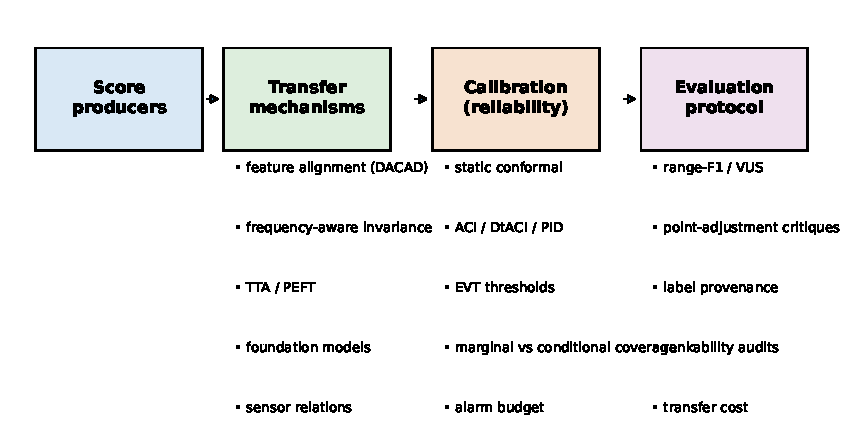
\includegraphics[width=\columnwidth]{fig_taxonomy.pdf}
\caption{Transfer mechanisms for cross-domain industrial anomaly detection, with representative citations per branch. Reliability (calibration) is deliberately drawn as a separate, orthogonal layer.}
\label{fig:taxonomy}
\end{figure}

\subsection{Feature Alignment and Discrepancy Minimization}
The mainstream approach learns representations whose source/target marginals match: adversarial alignment, maximum-mean-discrepancy variants with source weighting \cite{2310_14790}, contrastive objectives with anomaly injection \cite{dacad2024,2411_00914}, and source-free variants that adapt without source data \cite{2503_08749}. These methods produce competitive results on leave-one-condition-out benchmarks, but two failure modes recur across domains: alignment in feature space is frequency-agnostic, so it can erase band-specific fault signatures \cite{freqmatters2025}; and when the label spaces differ (anomaly-injection taxonomies do not transfer), contrastive gains shrink---in leave-one-industry-out settings, feature-space alignment has not consistently beaten plain reconstruction baselines \cite{2503_23060}.

\subsection{Frequency-Aware Invariance}
A newer branch makes spectral structure explicit: frequency-guidance losses for multi-source domain generalization in bearing diagnosis \cite{2502_00545}, band-level consistency objectives, and diagnostic studies that isolate spectral shift as a failure driver \cite{freqmatters2025,foundational2025}. The design question this branch confronts is preservation: aligning spectral statistics across domains can remove the very bands in which target faults live, motivating objectives that align domain-common bands while preserving saliency of fault-specific ones. In our own leave-one-industry-out benchmark \cite{our_scc}, such invariant objectives were neutral at attainable scales---an honest negative result that the branch must address with controlled shift gradients rather than null ablations.

\subsection{Test-Time Adaptation and Parameter-Efficient Adaptation}
TTA updates a small part of the model at deployment using unlabeled target data: low-rank input/output calibrators with frequency and robustness losses \cite{petsa2025}, normalization-statistic adaptation, concept-drift-aware online objectives \cite{2412_08435}, and TTA designed specifically for unsupervised time-series anomaly detection \cite{2312_11976}. Related streaming methods use regime detection to schedule adaptation \cite{2603_27814,2604_01845}. A recurring safety issue: in anomaly detection, adapting on the test stream can absorb the anomalies themselves into ``normal''---the adaptation objective must actively avoid explaining faults, not merely chase low reconstruction error \cite{2312_11976}.

\subsection{Foundation Models and Zero-Shot Transfer}
Time-series foundation models promise zero-shot transfer \cite{chronos2024}; critiques find their advantages narrow on shifted industrial series, where spectral coverage and domain diversity decide outcomes \cite{freqmatters2025,foundational2025,2502_03383,2510_26777}. Context-parroting baselines and simple forecasters remain tough to beat \cite{2505_11349}; industrial-specific foundations are emerging for bearings \cite{2504_01373} and as retrieval/agent systems \cite{2506_02081}. In our 6-fold benchmark \cite{our_scc}, a zero-shot foundation model (Chronos-bolt-small) transferred as a score producer but was matched or beaten by a 1.3M-parameter reconstruction encoder on five of six domain families---evidence that \emph{transfer mechanism} and \emph{model size} should be evaluated orthogonally.

\subsection{Sensor-Relation and Graph Structure}
Physical coupling among sensors is a transferable structural prior: graph anomaly detection formalisms \cite{2302_00058,2307_03759}, adaptive segmentation with structural features for rotating machinery \cite{2504_20756}, and relation-consistency objectives that penalize divergence of cross-channel dependency structure between domains. These methods are attractive when channel sets overlap; under disjoint sensor sets the relation structure must be constructed from physical roles rather than learned names, and relation alignment reduces to designing an equivariant channel embedding---an open design problem.

\section{Reliability and Calibration}
\label{sec:calibration}

A detector that outputs scores is not yet a monitor; something must turn scores into alarms. This section surveys the machinery that makes the \emph{threshold} reliable, and the failure modes specific to cross-domain deployment.

\subsection{Conformal Prediction Foundations}
Split conformal prediction turns any score into a threshold with finite-sample marginal coverage on exchangeable data \cite{lei2018}. Exchangeability fails for time series (serial dependence) and, more severely, for cross-domain deployment (the target is a different population). The conformal time-series literature addresses the first failure: sequential predictive conformal inference \cite{2212_03463}, copula- and kernel-based multi-step variants \cite{2212_03281,2405_16828}, decomposition-aware calibration \cite{2406_16766}, joint adaptive region estimation \cite{2407_06390}, normalizing-flow and modern-Hopfield calibration \cite{2502_05709,2303_12783}, relational calibration for correlated series \cite{2502_09443}, and change-point-aware and deep-sequence variants \cite{2509_02844,2610_02357,2609_33868}. Adaptive conformal inference (ACI) replaces exchangeability with online feedback and gives long-run coverage under arbitrary dependence \cite{aci2021}; multiplicative/additive update rules \cite{dtaci2022} and PID-control formulations \cite{conformalpid2023} refine its dynamics. Extreme-value thresholding is the classical streaming alternative, controlling tail exceedance with a generalized-Pareto fit \cite{siffer2017}.

\subsection{Calibration Under Domain (Not Just Temporal) Shift}
Cross-domain calibration is much less studied than cross-time calibration. The relevant questions are: does a source-calibrated threshold transfer at all; and what does it cost to force coverage on the target? Our six-fold, four-domain-family benchmarking study \cite{our_scc} answers both empirically: static source thresholds fail in \emph{both} directions across every fold (normal-window coverage spanning $0.18$--$0.999$ at a nominal $0.90$), while online ACI restores coverage to within $0.015$ on five of six folds at negligible cost; the transfer cost is measurable as interval inflation ($0.5\times$--$19\times$), though a band-spectral divergence statistic does not predict it. Two negative results from that study generalize beyond the specific benchmark: a divergence-shifted quantile adds nothing over plain ACI, and a divergence-conditioned (Mondrian) quantile is consistently slightly worse.

\subsection{The Alarm-Budget Problem}
Online conformal rules guarantee the \emph{stream-wide} alarm rate, not the normal-window false-positive rate; when anomalies are abundant and strongly separable, the budget is consumed by true anomalies and normal-window coverage over-shoots. This alarm-budget effect is the cross-domain calibration problem that single-domain studies rarely encounter, because anomaly prevalence in deployment differs from the calibrated regime. A normal-anchored variant \cite{our_scc}---updating the quantile only on likely-normal windows, with an exclusion threshold $\kappa q_t$---fixes the defect: detection rates on anomaly-rich folds rise several-fold at matched normal-window FPR, while anomaly-sparse folds recover plain ACI. Open theory questions remain (below).

\subsection{Calibration Meets Foundation Models}
Foundation-model forecasts can serve as nonconformity scores for conformal prediction \cite{2507_08858}, and retrieval-augmented or agent-based pipelines increasingly bundle scoring and calibration \cite{2506_02081}. Our benchmarking study contributes a caution that applies to every score producer, classical or foundation: \emph{calibration quality and ranking quality decouple}. Coverage can be restored even when the score ranks anomalies below chance---in which case the alarms are calibrated and useless. Deployments should therefore audit rankability (a feature-baseline AUROC suffices) before trusting any calibration layer.

\begin{table}[t]
\caption{Calibration methods for cross-domain deployment, with scope and known failure modes.}
\label{tab:calibration}
\centering
\small
\begin{tabular}{p{2.3cm}p{2.4cm}p{2.9cm}}
\toprule
Method family & Addresses & Known failure mode \\
\midrule
Static split conformal \cite{lei2018} & exchangeable data & fails under any cross-domain shift (both directions) \\
EVT/tail fits \cite{siffer2017} & streaming, stationary tail & source-calibrated; inherits static failure \\
ACI \cite{aci2021}, DtACI \cite{dtaci2022}, CP-PID \cite{conformalpid2023} & temporal drift, long-run rate & stream-level budget; over-covers when anomalies abundant \\
Mondrian/conditional variants & subpopulation coverage & small feedback samples; no gain in cross-domain benchmarks \\
NA-ACI (normal-anchored) & alarm-budget allocation under shift & assumes anomaly-pure exclusion tail; $\kappa$ trade-off \\
\bottomrule
\end{tabular}
\end{table}

\section{Evaluation Practices and Pitfalls}
\label{sec:evaluation}

Cross-domain anomaly detection is unusually easy to evaluate dishonestly by accident. We collect the specific, documented pitfalls a cross-domain study must handle.

\subsection{Metrics: The Point-Adjustment Debate and Its Aftermath}
Point-wise metrics dominated early work and were inflated by point-adjustment (counting any alarm inside an anomalous segment as correct). A line of critique work showed that adjustment can make random detectors look excellent \cite{2109_05257,2308_13068}, proposed unbiased protocols and range-aware metrics \cite{2405_12096,2305_09691}, revisited the ranking behavior of widely used datasets \cite{2603_18985}, and recently stress-tested the post-adjustment evaluation landscape itself \cite{2607_11969}. The field has largely migrated to range-based $F_1$ and VUS, but cross-domain studies add a distinct requirement: since label spaces differ across domains, the \emph{transferable} metrics are score-calibration metrics (coverage, false-alarm rate, interval inflation) plus rank metrics evaluated per target domain---not cross-domain accuracy of a shared classifier.

\subsection{Label and Protocol Provenance}
Benchmark labels arrive as seeded faults, status codes, run-to-failure conventions, or synthetic injections. Each carries a distinct bias: seeded-fault datasets undersample natural degradation; run-to-failure windows are temporally correlated and degradation-ordered; synthetic injections assume separability by construction. Two pathologies we documented empirically \cite{our_scc} deserve special mention. First, \emph{below-chance rankings}: under some labeling protocols, model scores---and even simple feature baselines and zero-shot foundation models---rank anomalous windows below normal ones, because the labeled period differs from normal windows in amplitude or spectral statistics rather than in reconstructability. Second, \emph{alarm-budget illusions}: coverage can look nominal while detection utility is zero. Both pathologies argue for mandatory rankability audits and operational metrics (false alarms per hour, detection delay) alongside calibration numbers.

\subsection{Protocol Desiderata for Cross-Domain Claims}
Synthesizing the critique literature \cite{2109_05257,2409_13053,2511_18739,2405_12096} and our benchmarking experience \cite{our_scc}, we propose the following minimum protocol for cross-domain industrial anomaly detection papers: (i) leave-one-\emph{domain} (ideally leave-one-industry) out, not random splits; (ii) preserve native sampling rates, or evaluate the resampling choice explicitly; (iii) document how every anomaly label was produced and state the protocol's limitations; (iv) report rank metrics with a cheap feature-baseline audit; (v) report a calibration layer with nominal level, achieved coverage, and false-alarm rates separately; (vi) report transfer cost (e.g., interval inflation) so that reliability is priced; and (vii) fix seeds and report seed spread. Most of these are cheap; their absence---not compute---is the main reproducibility gap in the current literature.

\subsection{Classical Baselines and the Reproducibility Baseline}
Comparisons against deep models should include strong classical baselines; several studies find that well-tuned classical detectors remain competitive on industrial streams \cite{2204_01637,2212_11080}, and reconstructed simple baselines (e.g., PCA or feature-Mahalanobis scores) calibrate and rank surprisingly well across domain families. We treat such baselines as mandatory rather than optional in cross-domain evaluations, because they bound how much of the reported gain is attributable to transfer machinery versus score-producer capacity.

\section{Open Problems}
\label{sec:open}

\textbf{Conditional coverage under domain shift.} Marginal coverage is now attainable cross-domain with online conformal methods, but conditional (group- or regime-wise) coverage is not: conditional variants tested to date---Mondrian binning, divergence conditioning---either shrink feedback samples or fail to capture the conditioning that matters \cite{2502_09443,2609_33868}. A principled conditioning variable, and theory connecting measurable diagnostics (exclusion rates, score-distribution drift) to conditional coverage bounds, remain open.

\textbf{Alarm-budget-aware calibration.} The normal-anchored ACI variant resolves the budget allocation empirically, but its exclusion assumption is heuristic; formalizing budget-aware conformal rules---with guarantees that degrade gracefully when anomalies are not separable---is a well-posed theory problem with immediate deployment value in any stream whose anomaly prevalence is unknown \cite{aci2021,2506_15831}.

\textbf{Real process- and mining-industry benchmarks.} The absence of public mining SCADA data and the thinness of semiconductor process benchmarks shape what the field can claim. Fleet-scale corpora \cite{2605_09081} and cross-domain suites \cite{2503_23060} are first steps; what is missing is labeled, native-rate, multi-industry data with documented provenance, plus an evaluation standard \cite{2511_18739} that makes claims comparable.

\textbf{Foundation models versus transfer mechanisms.} Zero-shot foundation models transfer as score producers but do not automatically dominate small domain models on shifted industrial series \cite{freqmatters2025,foundational2025,2505_11349}; understanding \emph{when} scale substitutes for adaptation---and how to combine both---is open, and requires orthogonal evaluations of model capacity and transfer mechanism.

\textbf{Safety of test-time adaptation in monitoring.} TTA objectives can absorb anomalies into the normal model; robust TTA for anomaly detection must actively preserve novelty, not merely reduce reconstruction error \cite{2312_11976,2604_01845}. Criteria and audits for ``adaptation safety'' in monitoring deployments are not yet standardized.

\textbf{Concept drift meets domain shift.} Temporal drift and cross-domain shift are usually studied separately \cite{2506_15831,2412_08435}; real deployments face both, and calibration feedback (alarm-rate control) interacts with drift detectors in ways that are not understood. Joint protocols that vary both axes are a promising empirical direction.

\section{Conclusion}
\label{sec:conclusion}

Cross-domain industrial anomaly detection has matured from per-machine modeling to a literature with a recognizable stack: score producers, transfer mechanisms, calibration layers, and evaluation protocols. This survey argued that the field's center of gravity should shift toward the last two layers. Transfer mechanisms---feature alignment, frequency-aware invariance, test-time adaptation, foundation models, sensor-relation structure---deliver gains that are real but domain-dependent; calibration is where cross-domain deployment is won or lost, because static thresholds fail everywhere, online adaptive conformal methods restore coverage at negligible cost, and the transfer cost is measurable even when it is not predictable. Evaluation, finally, is where the field most often misleads itself: point adjustment is no longer the only trap---below-chance rankings, alarm-budget illusions, and label-protocol bias are systematic. We hope the protocol desiderata and the negative results collected here help the next wave of cross-industry monitoring systems be evaluated the way they will be deployed.


\bibliographystyle{IEEEtran}
\bibliography{references}

\end{document}
